%! TEX program = lualatex
\documentclass[12pt]{scrartcl}
% Packages
%\usepackage[margin=1.5in]{geometry}
\usepackage{index}
\makeindex
\usepackage{amsbsy} % Bold math symbols
\usepackage{tcolorbox}
\tcbuselibrary{theorems}
\tcbuselibrary{skins}
\tcbuselibrary{breakable}
\usepackage{varwidth}
\usepackage{textcomp}
\usepackage{amsmath}
\usepackage{esint}
\usepackage{titlesec}
\usepackage{xcolor}
\usepackage{titling}
\usepackage[linktocpage]{hyperref}
\usepackage{pgfplots}
\usepackage{multicol}
\setlength{\columnsep}{2em}
\usepackage{caption}
\usepackage{amsthm}
\usepackage{import}
\usepackage{cancel}
\usepackage{caption}
\usepackage{nicematrix}
\usepackage{enumerate}
\usepackage{graphicx}
\usepackage[italian]{babel}
\usepackage{setspace}
\setstretch{1.2}
% To reset footnote numbering each page
\usepackage[perpage]{footmisc}
\hypersetup{colorlinks,breaklinks, linkcolor=[RGB]{133,68,66}}
\definecolor{mastercolor}{HTML}{854442}


% Titles 
\title{Appunti di\\ \vspace{.3cm} Analisi 3}
\author{Manuel Deodato}
\date{}




\newtheoremstyle{style}% name of the style to be used
{5pt}% measure of space to leave above the theorem. E.g.: 3pt
{5pt}% measure of space to leave below the theorem. E.g.: 3pt
{\normalfont}% name of font to use in the body of the theorem
%{15pt}% measure of space to indent
{0pt}% measure of space to indent
{\noindent\sffamily\bfseries}% name of head font
{}% punctuation between head and body
{ }% space after theorem head; " " = normal interword space
{\thmname{#1}\thmnumber{ #2}{\thmnote{ (#3)}.\ }}


\theoremstyle{style}
\newtheorem{esempio}{Esempio}[section]
\newtheorem{definizione}{Definizione}[section]
\newtheorem{prop}{Proposizione}[section]
\newtheorem{teorema}{Teorema}[section]
\newtheorem{lemma}{Lemma}[teorema]
\newtheorem{corollario}{Corollario}[teorema]
\newtheorem{osservazione}{Osservazione}[section]
\newtheorem{notazione}{Notazione}[section]
\newtheorem{esercizio}{Esercizio}[section]





\tcolorboxenvironment{definizione}{blanker,breakable,left=5mm,before skip=10pt,after skip=10pt, borderline west={.5mm}{0pt}{mastercolor}, before upper={\setlength{\parindent}{15pt}}}
\tcolorboxenvironment{lemma}{blanker,breakable,left=5mm,before skip=10pt,after skip=10pt, borderline west={.5mm}{0pt}{mastercolor}, before upper={\setlength{\parindent}{15pt}}}
\tcolorboxenvironment{teorema}{enhanced,blanker,breakable,left=5mm,before skip=10pt,after skip=10pt, borderline west={.5mm}{0pt}{mastercolor}, before upper={\setlength{\parindent}{15pt}}}
\tcolorboxenvironment{corollario}{blanker,breakable,left=5mm,before skip=10pt,after skip=10pt, borderline west={.5mm}{0pt}{mastercolor}, before upper={\setlength{\parindent}{15pt}}}
\tcolorboxenvironment{prop}{blanker,breakable,left=5mm,before skip=10pt,after skip=10pt, borderline west={.5mm}{0pt}{mastercolor}, before upper={\setlength{\parindent}{15pt}}}
\tcolorboxenvironment{esempio}{blanker,breakable,left=5mm,before skip=10pt,after skip=10pt, borderline west={.5mm}{0pt}{mastercolor}, before upper={\setlength{\parindent}{15pt}}}
\tcolorboxenvironment{esercizio}{blanker,breakable,left=5mm,before skip=10pt,after skip=10pt, borderline west={.5mm}{0pt}{mastercolor}, before upper={\setlength{\parindent}{15pt}}}
\tcolorboxenvironment{osservazione}{blanker,breakable,left=5mm,before skip=10pt,after skip=10pt, borderline west={.5mm}{0pt}{mastercolor}, before upper={\setlength{\parindent}{15pt}}}

\newenvironment{svolgimento}{\renewcommand\qedsymbol{$\blacksquare$}\begin{proof}[Svolgimento]}{\end{proof}}

%% Generic box
\newtcolorbox{eqbox}[1][]
{
colback=gray!10,
arc=0pt,
boxrule=0pt,
title=#1
}

 \newenvironment{boxenv}[1][]{
    \begin{eqbox}[#1]
    }{
   \end{eqbox}
}



%Captions
\captionsetup[figure]{font=footnotesize,labelfont=footnotesize}
\captionsetup[table]{font=footnotesize,labelfont=footnotesize}
%Titlesec
\titleformat{\section}
{\fontsize{20}{20}\scshape}
{{\color{mastercolor}\fontsize{30}{20}\selectfont\thesection}}
{0.7em}
{}
\titlespacing*{\section}{0pt}{*2}{1cm}
\titlespacing*{\subsection}{0pt}{*5}{.25cm}
\titlespacing*{\subsubsection}{0pt}{*4.5}{.25cm}

% Personalizza la formattazione della subsection
\titleformat{\subsection}[block]{\centering\fontsize{15}{20}\bfseries}{\color{mastercolor}\thesubsection}{.5em}{}


% Personalizza la formattazione della subsubsection
\titleformat{\subsubsection}[block]{\centering\fontsize{13}{10}\bfseries}{\color{mastercolor}\thesubsubsection}{.5em}{}

% Maketitle customization
\renewcommand{\maketitle}{
\begin{center}
{\sffamily
{\fontsize{20}{20}\selectfont\MakeUppercase{\thetitle}}}

\vspace{0.2in}

{\large\MakeUppercase{\theauthor}}
\end{center}
}

%Evaluate symbol
\DeclareMathOperator{\di}{d\!}
\newcommand*\Eval[3]{\left.#1\right\rvert_{#2}^{#3}}

%%%%%%% Numero delle equazioni in formato a.b
\numberwithin{equation}{subsection}
%%%%%

%%%%%%%%%% Personalizzazione numeri lista
\renewcommand{\theenumi}{(\arabic{enumi})}

%%%% Table of contents

\usepackage[titles]{tocloft}

\renewcommand{\cftdot}{}
\usepackage{titletoc}
%\setcounter{tocdepth}{2}

%%%%%%%%%%%%%%%% Toc style

% Personalizzazione scritta indice


% Font
\renewcommand{\textbf}[1]{\textsf{\bfseries #1}}
\usepackage{fontspec}
\usepackage{unicode-math}
\usepackage[default]{fontsetup}



%%% Hook
\newcommand{\longhookrightarrow}{\lhook\joinrel\longrightarrow}


\begin{document}
\maketitle
\vspace{6cm}
\begin{center}
		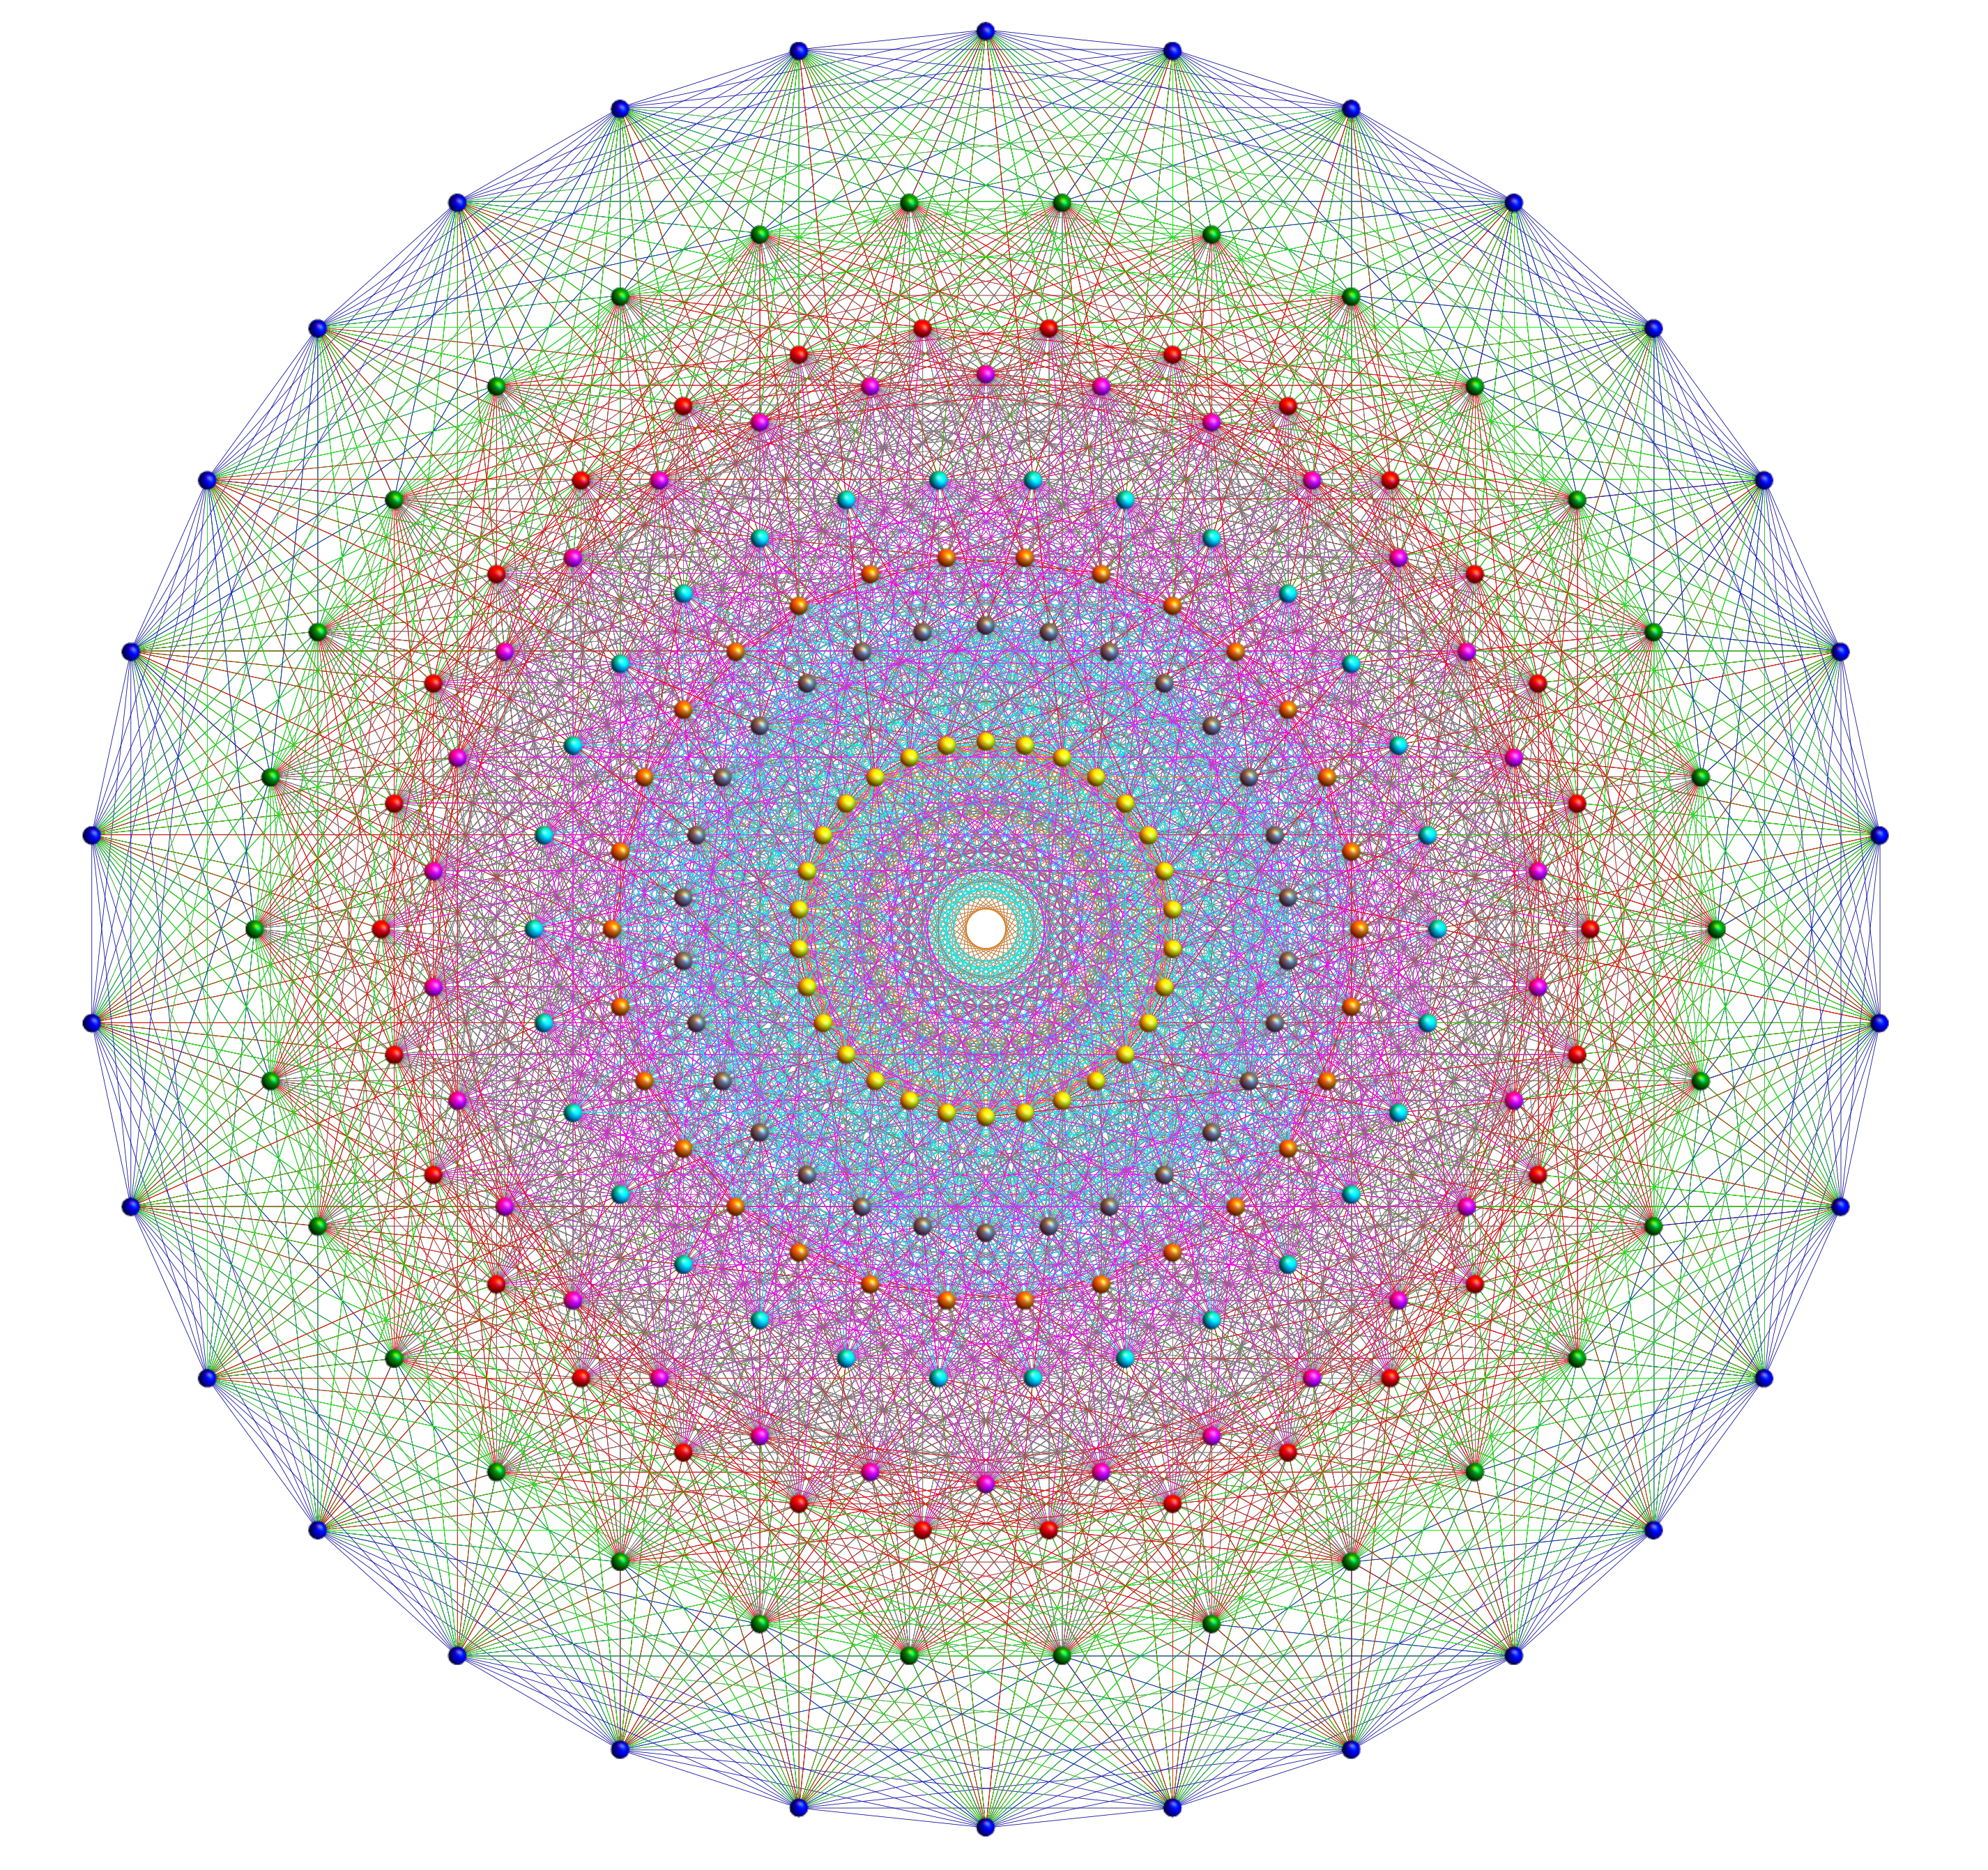
\includegraphics[width=.8\columnwidth]{front.jpg}
\end{center}
\newpage
\tableofcontents
\newpage
\section{Teoria della misura e dell'integrazione}
Si costruisce una teoria della misura per spazi euclidei che sia compatibile con i teoremi di passaggio al limite sotto il segno di integrale.
\subsection{Misura esterna}
Si considerano gli oggetti fondamentali di $\mathbb{R}^d$, al variare di $d$, cio\`e, rettangoli per $d=2$, parallelepipedi per $d=3$ e cos\`i via.
Questi sono della forma
\[
I = \prod_{i=1} ^d (a_i, b_i) \subseteq \mathbb{R}^d
\] 
con $-\infty<a_i < b_i < +\infty$, dove ogni $(a_i,b_i) \subset \mathbb{R}$ \`e un intervallo reale.
Il loro volume \`e dato da
\[
\lvert I \rvert = \prod_{i=1} ^d (b_i -a_i)
\] 
\begin{definizione}
	[Misura esterna]
	Sia $E \subseteq \mathbb{R}^d$ un sottoinsieme generico. 
	Dato un suo generico ricoprimento di plurintervalli chiusi $S= \left\{ I_k \right\} _{k=1} ^{\infty} $ e data la funzione
	\[
	\sigma (S) = \sum_{k=1}^{+\infty} \lvert I_k \rvert 
	\] 
	si definisce la misura esterna di $E$ come
	\[
	\lvert E \rvert _e := \inf_S \sigma (S) 
	\] 
	che ha valori in $[0,+\infty]$.
\end{definizione}
\begin{osservazione}
Questa funzione misura esterna \`e ben definita su $\mathcal{P} (\mathbb{R}^d)$, cio\`e su ogni possibile sottoinsieme di $\mathbb{R}^d$ e ha valori in $[0,+\infty]$.
Per costruire una buona misura e arrivare alla misura di Lebesegue, si vorr\`a limitare l'intervallo di definizione della misura esterna ad una certa porzione di \textit{sottoinsiemi buoni} di $\mathbb{R}^d$, che si chiameranno \textit{insiemi misurabili} (secondo Lebesgue).
\end{osservazione}
\noindent Ora si analizzano alcune propriet\`a della misura esterna.
\begin{definizione}
	[Insiemi non sovrapposti]
	Dati due plurintervalli $I_k, I_j$, questi si dicono \textit{non sovrapposti} se $\mathring{I}_k\cap \mathring{I_j} = \varnothing$, per $k \neq j$, cio\`e la frontiera non conta. 
\end{definizione}
\begin{teorema}
	Sia $I$ un plurintervallo; allora $\lvert I \rvert_e = \lvert I \rvert $, cio\`e la misura esterna coincide con la misura usuale.
\end{teorema}
\begin{teorema}
	Siano $A, B \subseteq \mathbb{R}^d$, con $A \subseteq B$; allora $\lvert A \rvert _e \le \lvert B \rvert _e$.
\end{teorema}
\begin{corollario}
	Siano $E,E' \subseteq \mathbb{R}^d$, con $E'\subseteq E$ e $\lvert E \rvert _e = 0$; allora $\lvert E' \rvert _e =0$.
\end{corollario}
\noindent Da queste prime propriet\`a, si pu\`o vedere che, dato un insieme numerabile di $\mathbb{R}^d$ 
\[
E = \bigcup_{k=1} ^{+\infty} \left\{ x_k \right\} , \ x_k \in \mathbb{R}^d
\] 
allora $\lvert E \rvert _e = 0$.
\begin{proof}
	Fissato $\varepsilon >0$, si trova un ricoprimento di $E$ dato da $S_\varepsilon = \left\{ I_k \right\} _{k=1} ^{+\infty} $ tale che $\lvert I_k \rvert = \varepsilon  / 2^k$; allora
	\[
	\sigma (S_\varepsilon ) = \sum_{k=1}^{+\infty} \lvert I_k \rvert =\varepsilon \sum_{k=1}^{+\infty} \frac{1}{2^k} = \varepsilon 
	\] 
	quindi, per definizione:
	\[
	\lvert E \rvert _e \le \sigma (S_\varepsilon ) = \varepsilon 
	\] 
	quindi si pu\`o rendere piccola a piacere, da cui la tesi.
\end{proof}
\noindent Da questa osservazione, segue direttamente che l'insieme dei numeri razionali \`e un insieme \textit{piccolo}, nel senso che ha misura esterna nulla.
\begin{teorema}\label{tdmt1}
	Sia $E \subseteq \mathbb{R}^d$; allora, fissato $\varepsilon > 0$, si trova un insieme aperto $G \subseteq \mathbb{R}^d$ tale che $E \subseteq G$ e 
	\[
	\lvert G \rvert _e \le  \lvert E \rvert _e + \varepsilon 
	\] 
\end{teorema}
\begin{proof}
Sia $\varepsilon > 0$ fissato; allora esiste un ricoprimento chiuso $S_\varepsilon = \left\{ I_ k\right\}_{k=1} ^{+\infty}  $ di $E$ tale che 
\[
\sigma (S_\varepsilon ) = \sum_{k=1}^{+\infty} \lvert I_k \rvert \le \lvert E \rvert _e + \frac{\varepsilon}{2} 
\] 
Tale ricoprimento esiste perch\'e, per definizione
\[
\lvert E \rvert _e = \inf_S \sigma (S)
\] 
quindi si pu\`o prendere il ricoprimento che soddisfa tale estremo inferiore e \textit{allargarlo di} $\varepsilon $.
Ora si costruiscono degli intervalli $I_k^*$ tali che $I_k \subset \mathring{I}_k^*$ e che
\[
\lvert I_k ^*\rvert \le \lvert I_k \rvert + \frac{\varepsilon }{2^{k+1} }
\] 
per cui si pu\`o definire
\[
	G := \bigcup_{k=1} ^{+\infty} \mathring{I}^*_k
\] 
che \`e aperto perch\'e tutti gli $\mathring{I}_k^*$ sono aperti.
Si vede che soddisfa $E \subset G$ per costruzione e
\[
\lvert G \rvert _e \le \sum_{k=1}^{+\infty} \lvert I_k^* \rvert \le \sum_{k=1}^{+\infty} \lvert I_k \rvert +\varepsilon \sum_{k=1}^{+\infty} \frac{1}{2^{k+1} } \le \lvert E \rvert _e + \frac{\varepsilon }{2}+ \frac{\varepsilon }{2}=\lvert E \rvert _e + \varepsilon 
\] 
da cui la tesi.
\end{proof}
\begin{teorema}
	Sia $E \subseteq \mathbb{R}^d$; allora $\exists H \subseteq \mathbb{R}^d$ della forma
	\[
	H = \bigcap_{j=1} ^{+\infty} G_j
	\] 
	con $G_j$ aperti, tale che $E \subseteq H$ e $\lvert E \rvert _e = \lvert H \rvert _e$.
\end{teorema}
\begin{proof}
	Per il teorema precedente (\ref{tdmt1}), dato $\varepsilon = 1/k$, si trova una famiglia numerabile di aperti $G_k \supseteq E $ tali che
	\[
	\lvert G_k \rvert _e \le  \lvert E \rvert _e + \frac{1}{k}
	\] 
	Preso $H := \bigcap_{k=1} ^{+\infty}  G_k$, allora $G_k\supseteq H \supseteq E,\ \forall k$, quindi 
	\[
		\lvert E \rvert _e \le \lvert H \rvert_e \le \lvert G_k \rvert _e \le \lvert E \rvert _e + \frac{1}{k}
	\] 
	Prendendo il limite per $k\to +\infty$, visto che $\lvert E \rvert _e$ e $\lvert H \rvert _e$ non dipendono da $k$, si rimane con $\lvert E \rvert _e \le \lvert H \rvert _e \le \lvert E \rvert _e$, da cui la tesi.
\end{proof}
\begin{osservazione}
Un insieme ottenuto come intersezione numerabile di aperti \`e chiamato $G_\delta $; il teorema sopra, quindi, permette di trovare sempre un certo insieme $G_\delta $ che ha stessa misura dell'insieme in questione e lo contiene.
Il vantaggio \`e legato alla struttura che gli insiemi $G_\delta $ hanno rispetto a sottoinsiemi generici di $\mathbb{R}^d$, che spesso \`e preferibile.
Si nota, infine, che insiemi ottenuti come unione numerabile di chiusi si indica con $F_\sigma $.
\end{osservazione}
\subsection{Misurabilit\`a}
\begin{definizione}
	[Insieme misurabile]
	Un insieme $E \subseteq \mathbb{R}^d$ si dice \textit{misurabile secondo Lebesgue} se $\forall \varepsilon >0$, $\exists G \subseteq \mathbb{R}^d$ aperto, con $G\supseteq E$, tale che $\lvert G \setminus E \rvert _e < \varepsilon $.
	In questo caso, la misura di $E$ \`e data da $\lvert E \rvert := \lvert E \rvert _e$.
\end{definizione}
\noindent Di seguito, si enunciano alcune propriet\`a degli insiemi misurabili.
\begin{prop}
Se $E \subseteq \mathbb{R}^d$ \`e aperto, allora \`e misurabile.
Inoltre, se $E \subseteq \mathbb{R}^d$ \`e tale che $\lvert E \rvert _e = 0$, allora \`e misurabile.
\end{prop}
\begin{proof}
	Per vedere il secondo punto, si osserva che, per il teorema \ref{tdmt1}, si trova un aperto $E\subseteq G \subseteq \mathbb{R}^d$ tale che $\lvert G \rvert _e \le \lvert E \rvert _e + \varepsilon =\varepsilon $, quindi\footnote{La prima disuguaglianza fa uso del fatto che $G \setminus E \subseteq G$.} $\lvert G\setminus E \rvert _e \le  \lvert G \rvert _e \le \varepsilon $.
\end{proof}
\begin{osservazione}
Si \`e visto che per $E\subseteq \mathbb{R}^d$, si pu\`o trovare sempre una aperto che lo contiene tale che $\lvert G \rvert _e \le  \lvert E \rvert _e + \varepsilon $, ma questa condizione non coincide con quella di misurabilit\`a.
Infatti, si nota che
\[
G = E \cup \big(G \setminus E \big) \implies \lvert G \rvert _e\le \lvert E \rvert _e + \lvert G \setminus E \rvert _e
\] 
ma non si riesce a dedurre che $\lvert G \setminus E \rvert _e < \varepsilon $.
\end{osservazione}
\begin{teorema}\label{tdmt2}
	Valgono i seguenti punti.
	\begin{enumerate}[(a).]
		\item Se $\left\{ E_k \right\} _{k=1} ^{+\infty} $ sono misurabili, allora $\bigcup_{k=1} ^{+\infty} E_k$ \`e misurabile.
		\item Se $F$ \`e chiuso, allora \`e misurabile.
		\item Se $I$ \`e un intervallo, allora $I = \mathring{I}\cup \partial I$ e $\lvert \partial I \rvert = 0$.
	\end{enumerate}
\end{teorema}
\noindent \textit{Dimostrazione \ref{tdmt2}a.} Visto che gli $E_k$ sono tutti misurabili, allora $\forall \varepsilon >0, \ \exists G_k\supset E_k$ aperto tale che $\lvert G_k\setminus E_k \rvert_e < \varepsilon / 2^k $; definendo
\[
G:= \bigcup _{k=1} ^{+\infty} G_k
\] 
questo \`e aperto per costruzione e\footnote{Infatti $\forall k, \ E_k \subset G_k \Rightarrow \bigcup_k E_k \subset \bigcup_k G_k$. Inoltre, $x \in G \setminus E$ implica che $\exists k_0$ tale che $x \in G_k$ e che $\forall k, \ x \not\in E_k$; allora $x \in \bigcup_k (G_k \setminus E_k)$ perch\'e $x \in G_{k_0} \setminus E_{k_0}$.}
\[
E_k \subset G_k \Rightarrow E \subset G \hspace{.2cm} ; \hspace{.5cm} G \setminus E \subset \bigcup _{k=1} ^{+\infty} \big(G_k \setminus E_k\big)
\] 
Allora 
\[
\lvert G \setminus E \rvert _e \le \sum_{k=1}^{+\infty} \lvert G_k \setminus E_k \rvert _e \le \sum_{k=1}^{+\infty} \frac{\varepsilon }{2^k} = \varepsilon 
\] 
da cui la tesi. \qed

\noindent Per dimostrare che ogni chiuso \`e misurabile (\ref{tdmt2}b), si usa il seguente lemma.
\begin{lemma}\label{tdml1}
Siano $E_1,E_2 \subseteq \mathbb{R}^d$ due sottoinsiemi tali che $d(E_1,E_2)>0$; allora $\lvert E_1\cup E_2 \rvert_e = \lvert E_1 \rvert _e + \lvert E_2 \rvert _e$
\end{lemma}
\begin{proof}
	Sia $\delta = d(E_1,E_2) > 0$; allora, nell'inf della definizione di $\lvert E_1\cup E_2 \rvert _e$, ciascun ricoprimento $S$  candidato all'essere l'estremo inferiore si pu\`o sostituire con un $S'$ tale che ogni rettangolo $I_k$ abbia diametro
	\[
	\operatorname{diam} I_k := \sup \left\{ \lvert x-y \rvert  \mid x, y \in I_k \right\} 
	\] 
	pari o inferiore a un certo arbitrario $\varepsilon < \delta$.
	Questo \`e sempre possibile farlo perch\'e si ha $\sigma (S) = \sigma (S')$, visto che si \`e solo spezzato ogni rettangolo in sotto-rettangoli pi\`u piccoli che, quindi, restituiscono stessa area di quelli originari.
	In questo modo, per\`o, non pu\`o esistere alcun rettangolo $I_k$ che sia tale da intersecare entrambi gli insiemi, quindi si pu\`o spezzare un ricoprimento $S$ in base a quale dei due insiemi tocca:
	\[
		\lvert E_1\cup E_2 \rvert _e = \inf_{S} \sigma (S) = \inf_{S_1,S_2} \big[\sigma (S_1) + \sigma (S_2)\big]  = \inf_{S_1} \sigma (S_1) + \inf_{S_2} \sigma (S_2) = \lvert E_1 \rvert _e   + \lvert E_2 \rvert _e
	\] 
	da cui la tesi.
\end{proof}
\noindent \textit{Dimostrazione \ref{tdmt2}b.} Si assume preliminarmente $F$ compatto, per poi estendere il risultato al caso generale.
Sia $G \subseteq \mathbb{R}^d$ un aperto contenente $F$ e tale che $\lvert G \rvert \le  \lvert F \rvert _e + \varepsilon $, per $\varepsilon  > 0$; si deve arrivare a mostrare che $\lvert G \setminus F \rvert _e < \varepsilon $.
Intanto si nota che, grazie alla compattezza di $F$, si pu\`o usare il lemma \ref{tdml1}:
\[
G = \big(G\setminus F \big)\cup F \implies \lvert G \rvert = \lvert F \rvert _e  + \lvert G \setminus F \rvert _e \implies \lvert G \setminus F \rvert _e = \lvert G \rvert - \lvert F \rvert _e
\] 
Ma visto che $\lvert G \rvert  \le  \lvert F \rvert _e + \varepsilon $, allora si ottiene la tesi.
Ora si deve estendere la dimostrazione a $F$ chiuso, senza la condizione che sia necessariamente limitato, quindi compatto; per farlo, si scrive
\[
F = \bigcup_{k=1} ^{+\infty} F_k = \bigcup_{k=1} ^{+\infty} \Big(F \cap \overline{B}_k(0)\Big) 
\] 
con $\overline{B}_k(0)$ palla chiusa di centro l'origine e raggio $k$.
Si nota che ogni $F_k$ \`e chiuso, perch\'e intersezione di chiusi, e limitato perch\'e $\overline{B}_k(0)$ \`e limitato.
Ne segue che ogni $F_k$ \`e compatto, quindi misurabile per quanto appena detto; per il teorema \ref{tdmt2}a, allora, anche $F$ \`e misurabile.\qed

Da questi risultati appena visti, si ottengono, come corollario, i seguenti punti.
\begin{corollario}\label{tdmc1}
	Valgono i seguenti punti.
	\begin{enumerate}[(a).]
		\item Se $A$ \`e misurabile, allora $\mathbb{R}^d \setminus A$ \`e misurabile.
		\item Se gli $A_i$ sono misurabili, allora $\bigcap_{i=1} ^{+\infty} A_i$ \`e misurabile.
		\item Se $E_1 \subset E_2$ sono misurabili, allora $\lvert E_2\setminus E_1 \rvert = \lvert E_2 \rvert - \lvert E_1 \rvert $ e, quindi, $E_2\setminus E_1$ \`e misurabile.
	\end{enumerate}
\end{corollario}
\noindent Il punto \ref{tdmc1}a permette di dimostrare il seguente risultato.
\begin{prop}\label{tdmp1}
	$E \subseteq \mathbb{R}^d$ \`e misurabile $\iff \forall \varepsilon >0 , \ \exists F \subseteq \mathbb{R}^d$ chiuso con $F \subset E$ tale che $\lvert E \setminus F \rvert < \varepsilon $.
\end{prop}
\begin{proof}
	Per il corollario \ref{tdmc1}a, $E$ \`e misurabile se e solo se $E^c$\footnote{Con $c$ all'apice si intende il complementare.} \`e misurabile, cio\`e se per ogni $\varepsilon >0$, si trova un aperto $G \supset E^c$ tale che $\lvert G \setminus E^c \rvert_e < \varepsilon $.
	Ora, $G$ \`e aperto, quindi misurabile e, dunque, il suo complementare $F:= G^c$ \`e un chiuso misurabile. 
	Inoltre, visto che $E^c \subset G$, allora $E\supset F$ ed essendo $G \setminus E^c  = E \setminus F $, si ha la tesi.
\end{proof}
\begin{teorema}
	Sia $E \subseteq \mathbb{R}^d$; allora sono equivalenti i seguenti punti:
	\begin{enumerate}[(a).]
		\item $E$ \`e misurabile;
		\item $E = H \setminus Z$ con $\lvert Z \rvert =0$ e $H$ \`e un $G_\delta $;
		\item $E = H' \cup Z'$, con $\lvert Z' \rvert = 0$ e $H'$ \`e un $F_\sigma $.
	\end{enumerate}
\end{teorema}
\noindent Il seguente teorema fornisce una visione alternativa e pi\`u generale (perch\'e indipendente dalla struttura dello spazio in cui si lavora) per definire la misurabilit\`a.
\begin{teorema}
	[Teorema di Carath\'eodory]
	Un insieme $E \subseteq \mathbb{R}^d$ \`e misurabile se e solo se $\forall A \subseteq \mathbb{R}^d$, si ha
	\[
	\lvert A \rvert _e = \lvert A\cap E  \rvert _e + \lvert A\setminus E \rvert _e
	\] 
\end{teorema}
\begin{teorema}\label{tdmt3}
	Sia $\left\{ E_k \right\} _{k=1} ^{+\infty} $ una famiglia di sottoinsiemi misurabili di $\mathbb{R}^d$; allora valgono i seguenti punti:
	\begin{enumerate}[(a).]
		\item se $E_i \cap E_j = \varnothing$ per $i\neq j$, allora $\left\lvert \bigcup_{k=1} ^{+\infty} E_k \right\rvert = \sum_{k=1}^{+\infty} \lvert E_k \rvert $;
		\item se $E_k \nearrow E$, cioè $E_k \subseteq E_{k+1}$ per ogni $k$, definendo $E = \bigcup_{k=1} ^{+\infty} E_k$, allora $\lvert E \rvert =\displaystyle  \lim_{k \to +\infty} \lvert E_k \rvert $;
		\item se $E_k \searrow E$, cioè $E_{k+1} \subseteq E_k$ per ogni $k$, con $E = \bigcap_{k=1} ^{+\infty} E_k$, e se, inoltre, $\exists k : \lvert E_k \rvert < + \infty$, allora $\lvert E \rvert = \displaystyle \lim_{k \to +\infty} \lvert E_k \rvert $.
	\end{enumerate}
\end{teorema}
\noindent \textit{Dimostrazione \ref{tdmt3}a.} Per ogni $k$, si usa la prop. \ref{tdmp1} per dire che si trova un $F_k$ tale che $\lvert E_k \setminus F_k \rvert < \varepsilon  / 2^k$.
Visto che gli $F_k$ sono disgiunti per definizione, allora si pu\`o usare il lemma \ref{tdml1} per dire che
\[
	\left\lvert \bigcup_{k=1} ^m F_k\right\rvert = \sum_{k=1}^{m} \lvert F_k \rvert, \ \forall m \in \mathbb{N}
\] 
Inoltre
\[
\bigcup_{k=1} ^m F_k \subset \bigcup_{k=1} ^{+\infty} E_k \implies \sum_{k=1}^{m} \lvert F_k \rvert \le \left\lvert \bigcup_{k=1} ^{+\infty} E_k \right\rvert , \ \forall m \in \mathbb{N}
\] 
Visto che vale $\forall m \in \mathbb{N}$, allora \`e anche vero che
\[
\sum_{k=1}^{+\infty} \lvert F_k \rvert \le  \left\lvert \bigcup_{k=1} ^{+\infty} E_k \right\rvert 
\] 
da cui
\[
\left\lvert \bigcup_{k=1} ^{+\infty} E_k \right\rvert \ge \sum_{k=1}^{+\infty} \lvert F_k \rvert > \sum_{k=1}^{+\infty} \left(\lvert E_k \rvert -\frac{\varepsilon }{2^k}\right) = \sum_{k=1}^{+\infty} \lvert E_k \rvert - \varepsilon , \ \forall \varepsilon 
\] 
da cui $\left\lvert \bigcup_k E_k \right\rvert  \ge \sum_{k}^{} \lvert E_k \rvert $.
Al contempo, per\`o, \`e sempre vera la disuguaglianza
\[
\left\lvert \bigcup_{k=1} ^{+\infty} E_k\right\rvert \le \sum_{k=1}^{+\infty} \lvert E_k \rvert 
\] 
da cui la tesi. \qed

\noindent \textit{Dimostrazione \ref{tdmt3}b.} Visto che $\forall k, \ E_k \subseteq E_{k+1} $, si pu\`o definire equivalentemente 
\[
E := E_1 \cup \bigcup_{k=1} ^{+\infty} \big(E_{k+1} \setminus E_k\big)
\] 
in modo che siano tutti disgiunti. 
Si pu\`o, quindi, usare il corollario \ref{tdmc1}c, assumendo che $\forall k , \lvert E_k \rvert <+\infty$, e il punto \ref{tdmt3}a per scrivere che 
\[
\lvert E \rvert = \lvert E_1 \rvert + \sum_{k=1} ^{+\infty} \lvert E_{k+1} \setminus E_k \rvert = \lvert E_1 \rvert  +\sum_{k=1} ^{+\infty} \Big(\lvert E_{k+1}  \rvert - \lvert E_k \rvert \Big)
\] 
Questa espressione \`e tale da elidere ciascun termine tranne ``l'ultimo'', perci\`o:
\[
\lvert E \rvert = \lim_{k \to +\infty} \lvert E_k \rvert 
\] 
da cui la tesi.

Per dimostrarlo nel caso generale in cui non si assume che ogni $E_k$ abbia misura finita, si usa un'altra strada; intanto si definiscono gli $F_k := E_{k}\setminus E_{k-1}  $, con $E_0=\varnothing$, per cui 
\[
E = \bigcup_{k=1} ^{+\infty} F_k
\] 
Ora, gli $F_k$ sono a due a due disgiunti, pertanto si pu\`o usare il punto \ref{tdmt3}a per scrivere che
\[
\lvert E \rvert = \sum_{k=1} ^{+\infty} \lvert F_k \rvert 
\] 
In maniera del tutto analoga, si ha che
\[
E_n = \bigcup_{k=1} ^n F_k \implies \lvert E_n \rvert = \sum_{k=1}^{n} \lvert F_k \rvert 
\] 
Prendendo il limite di questa espressione, si vede che 
\[
\lim_{n \to +\infty} \lvert E_n \rvert = \lim_{n \to +\infty} \sum_{k=1}^{n} \lvert F_k \rvert = \sum_{k=1}^{+\infty} \lvert F_k \rvert = \lvert E \rvert 
\] 
da cui la tesi. \qed 

\noindent \textit{Dimostrazione \ref{tdmt3}c.} Si usa il fatto che $\exists k_0 : E_{k_0} $ ha misura finita per ricondurre la dimostrazione al punto precedente, cio\`e al caso crescente.
Infatti, avendo tutti insiemi di misura finita da $k_0$ in poi e avendo definito $E$ come l'intersezione di questi, si pu\`o far partire tale intersezione direttamente da $k=k_0$.
A questo punto, per tradurre il caso (c) al caso (b), dopo aver rinominato gli indici prendendo $k_0 =1$ e tutti gli altri di seguito, si definisce 
\[
F_k := E_1 \setminus E_k
\] 
Visto che gli $E_k$ sono decrescenti, $F_k$ \`e crescente e, quindi, per il punto (b) e il corollario \ref{tdmc1}c:
\[
\lvert F \rvert = \lim_{k \to +\infty} \lvert E_1\setminus E_k \rvert = \lvert E_1 \rvert - \lim_{k \to +\infty}  \lvert E_k \rvert 
\] 
Per\`o si nota che 
\[
F = \lim_{k \to +\infty} E_1 \setminus E_k=E_1 \setminus E\implies \lvert F \rvert = \lvert E_1 \rvert - \lvert E \rvert 
\] 
Combinando le due espressioni, si ottiene la tesi.\qed
\subsection{Misurabilit\`a di funzioni}
\begin{definizione}
	[Misurabilit\`a di una funzione]
	Dato $E \subseteq \mathbb{R}^d$ misurabile, si dice che $f: E \to \mathbb{R}$ \`e una funzione \textit{misurabile} (secondo Lebesgue) se, $\forall a \in \mathbb{R}$, l'insieme $\left\{ x \in E  \mid f> a \right\} $ \`e misurabile.
\end{definizione}
\noindent Pi\`u semplicemente, la notazione per $\left\{ x \in E  \mid f > a \right\} $ si indicher\`a con $\left\{ f>a \right\} $.
\begin{prop}
	Sia $f$ misurabile; allora sono equivalenti i seguenti punti:
	\begin{enumerate}[(a).]
		\item $\left\{ f \ge a \right\} $ \`e misurabile;
		\item $\left\{ f < a \right\} $ \`e misurabile;
		\item $\left\{ f\le a \right\} $ \`e misurabile.
	\end{enumerate}
\end{prop}
\begin{osservazione}
La misurabilit\`a di una funzione, allora, \`e verificata anche per cambiamenti della funzione stessa su insiemi a misura nulla.
\end{osservazione}
\begin{prop}
	Siano $f,g$ due funzioni misurabili; allora:
	\begin{enumerate}[(a).]
		\item $f+c$ \`e misurabile;
		\item $cf$ \`e misurabile;
		\item $f+g$ \`e misurabile;
		\item $f / g$ \`e misurabile se $g\neq 0$ q.o. 
	\end{enumerate}
\end{prop}
\begin{teorema}
	Sia $\left\{ f_k \right\}_{k}  $ una successione di funzioni misurabili; allora $\sup_{k} f_k$ e $\inf_{k} f_k$ sono misurabili e anche 
	\[
	\limsup _{k} f_k \hspace{1cm} \liminf_k f_k
	\] 
	sono misurabili e, quindi, anche $\lim_{k} f_k$ \`e misurabile.
\end{teorema}
\begin{teorema}
	Sia $\phi \in C(\mathbb{R})$ e sia $f$ finita quasi ovunque; se $f$ \`e misurabile, allora $\phi \circ f$ \`e misurabile.
\end{teorema}
\noindent Alcuni esempi importanti di applicazione del teorema precedente \`e dato dalle funzioni $\phi \circ f$ della forma $\lvert f \rvert $, $\lvert f \rvert ^p$, oppure $f^+ = \max \left\{ f,0 \right\} $ e $f^- = \min \left\{ f,0 \right\} $, quindi con $f = f^+ - f^-$.
\begin{definizione}
	[Funzione semplice]
	Sia $f : E \subseteq \mathbb{R}^d \to  \mathbb{R}$; si dice che $f$ \`e \textit{semplice} se esistono $N \in \mathbb{N}$, $a_k \in \mathbb{R}$ e $E_k \subset E$ disgiunti tali che
	\[
	f(x) = \sum_{k=1}^{N} a_k \chi _{E_k} (x)
	\] 
\end{definizione}
\begin{prop}
	Data $f$ semplice, questa \`e misurabile $\iff$ gli insiemi $E_k$ sono misurabili.
\end{prop}
\begin{teorema}\label{mft1}
	Valgono i seguenti punti.
	\begin{enumerate}[(a).]
		\item Data $f: E \to \mathbb{R}$, questa \`e limite puntuale di funzioni semplici. 
			In altri termini, $\forall f : E \to \mathbb{R}$, esiste una successione $ \left\{ f_k \right\} $, con $f_k$ semplici, tale che $f_k(x) \to f(x), \ \forall x \in E$.
		\item Se $f\ge 0$, allora la successione al punto (a) si pu\`o costruire crescente, cio\`e tale che $f_k(x) \le  f_{k+1} (x)$.
		\item Se $f$ \`e misurabile, allora la successione al punto (a) si pu\`o scegliere in modo tale che le funzioni $f_k$ siano misurabili.
	\end{enumerate}
\end{teorema}
\noindent \textit{Dimostrazione \ref{mft1}b}. Sia $f\ge 0$; si definiscono gli intervalli 
\[
\left[ \frac{j-1}{2^k}, \ \frac{j}{2^k} \right] 
\] 
e si definisce la successione
\[
f_k(x) = \begin{cases}
	\displaystyle \frac{j-1}{2^k}&,\ \text{ se } \displaystyle \frac{j-1}{2^k}\le f(x) \le \frac{j}{2^k}\\
	\\
	k &,\ \text{ se } f\ge k
\end{cases}
\] 
con $j=1,\ldots, k2^k$. 
Allora, per definizione, si ha:
\[
	f_k(x) = \sum_{j=1}^{k 2^k} \frac{j-1}{2^k}\chi _{\left[ \frac{j-1}{2^k}\le f \le \frac{j}{2^k} \right] } + k \chi _{\left\{ f\ge k \right\} } 
\] 
\begin{boxenv}[]
	\centering\color{mastercolor} Riprendere dalla lezione 3
\end{boxenv}
\end{document}
